\documentclass[12pt, a4paper]{article}
% --- Packages ---
\usepackage[utf8]{inputenc}
\usepackage[T1]{fontenc}
\usepackage{geometry}
\geometry{top=2.5cm, bottom=2.5cm, left=2.5cm, right=2.5cm}
\usepackage{amsmath, amssymb, amsthm}
\usepackage{graphicx}
\usepackage{enumitem}
\usepackage{xcolor}
\usepackage{tikz}
\usetikzlibrary{shapes, arrows, positioning, calc, trees, backgrounds}
\usepackage[most]{tcolorbox}
\usepackage{hyperref}
\usepackage{float}
\usepackage{fancyhdr}
% --- Colors ---
\definecolor{deepblue}{RGB}{0, 51, 102}
\definecolor{lightgray}{RGB}{240, 240, 240}
\definecolor{accentcolor}{RGB}{204, 0, 0}
% --- Custom Environments ---
\newtcolorbox[auto counter]{problem}[2][]{%
    colback=white,
    colframe=deepblue,
    coltitle=white,
    fonttitle=\bfseries\large,
    title=Problem \thetcbcounter: #2,
    sharp corners,
    boxrule=0.8mm,
    #1
}
\newtcolorbox{solution}{%
    colback=lightgray!30,
    colframe=accentcolor!80,
    coltitle=white,
    fonttitle=\bfseries,
    title=Step-by-Step Solution,
    sharp corners=south,
    boxrule=0.5mm,
    breakable
}
\newtcolorbox{concept}[1][]{%
    colback=yellow!10,
    colframe=orange!80!black,
    title=Key Concept,
    fonttitle=\bfseries,
    #1
}
% --- Header/Footer ---
\pagestyle{fancy}
\fancyhf{}
\lhead{\textbf{Deep Reinforcement Learning}}
\rhead{Practice Problem Set}
\cfoot{\thepage}
% --- TikZ Styles ---
\tikzset{
    state/.style={circle, draw, minimum size=1cm, fill=blue!10, thick},
    action/.style={circle, draw, minimum size=0.5cm, fill=red!10, thick},
    netnode/.style={circle, draw, minimum size=0.8cm, fill=green!10},
    arrow/.style={->, >=stealth, thick},
    box/.style={rectangle, draw, minimum width=2cm, minimum height=1cm, fill=white, thick}
}
% --- Title Info ---
\title{\textbf{Deep Reinforcement Learning Practice Guide}\\
\large Numerical Problems \& Detailed Solutions}
\author{Comprehensive Exam Preparation}
\date{\today}
\begin{document}
\maketitle
\section*{Introduction}
This practice guide contains 10 distinct numerical and conceptual problems covering the spectrum of Deep Reinforcement Learning. The problems are designed to be challenging, similar to previous exam questions, with a heavy emphasis on deep learning integration (DQN, Policy Gradients, Actor-Critic) while establishing foundations with Bandits and MDPs.
Each problem includes a detailed, step-by-step solution to aid in understanding the mechanics of the algorithms.
\tableofcontents
\newpage
% --- Problems will be inserted here ---
\begin{problem}{Non-Stationary Bandits \& Exponential Moving Average}
Consider a 3-armed bandit problem where the true action values $q_*(a)$ change over time (non-stationary). You are using an $\epsilon$-greedy agent with $\epsilon=0.1$ and a constant step-size parameter $\alpha=0.5$.
At time step $t=1$, the estimated action values are $Q_1(1) = 2.0$, $Q_1(2) = 0.0$, and $Q_1(3) = 1.0$.
The agent selects action $A_1=1$ and receives a reward $R_1=2.0$.
At time step $t=2$, the environment shifts significantly. The true values become $q_*(1)=1.0$, $q_*(2)=5.0$, $q_*(3)=0.0$.
The agent selects action $A_2=2$ and receives a reward $R_2=5.0$.
At time step $t=3$, the agent selects action $A_3=1$ again and receives a reward $R_3=1.0$ (reflecting the new true value).
\begin{enumerate}[label=(\alph*)]
    \item Calculate the updated action-value estimates $Q_2(a)$ after the first step.
    \item Calculate the updated action-value estimates $Q_3(a)$ after the second step.
    \item Calculate the updated action-value estimates $Q_4(a)$ after the third step.
    \item Explain why a constant step-size $\alpha$ is preferred over the sample-average method ($1/n$) in this non-stationary setting.
\end{enumerate}
\end{problem}
\begin{solution}
\textbf{(a) Update after step $t=1$}
The update rule for a constant step-size $\alpha$ is given by:
\[ Q_{k+1}(A_k) = Q_k(A_k) + \alpha [R_k - Q_k(A_k)] \]
where $A_k$ is the action taken and $R_k$ is the reward received.
At $t=1$:
\begin{itemize}
    \item Action $A_1 = 1$.
    \item Reward $R_1 = 2.0$.
    \item Current estimate $Q_1(1) = 2.0$.
    \item $\alpha = 0.5$.
\end{itemize}
Update for action 1:
\[ Q_2(1) = Q_1(1) + 0.5 [2.0 - 2.0] = 2.0 + 0 = 2.0 \]
Estimates for other actions remain unchanged:
\[ Q_2(2) = 0.0, \quad Q_2(3) = 1.0 \]
\textbf{(b) Update after step $t=2$}
At $t=2$:
\begin{itemize}
    \item Action $A_2 = 2$.
    \item Reward $R_2 = 5.0$.
    \item Current estimate $Q_2(2) = 0.0$.
\end{itemize}
Update for action 2:
\[ Q_3(2) = Q_2(2) + 0.5 [5.0 - 0.0] = 0.0 + 2.5 = 2.5 \]
Estimates for other actions remain unchanged:
\[ Q_3(1) = 2.0, \quad Q_3(3) = 1.0 \]
\textbf{(c) Update after step $t=3$}
At $t=3$:
\begin{itemize}
    \item Action $A_3 = 1$.
    \item Reward $R_3 = 1.0$ (reflecting the new true value).
    \item Current estimate $Q_3(1) = 2.0$.
\end{itemize}
Update for action 1:
\[ Q_4(1) = Q_3(1) + 0.5 [1.0 - 2.0] = 2.0 + 0.5(-1.0) = 2.0 - 0.5 = 1.5 \]
Estimates for other actions remain unchanged:
\[ Q_4(2) = 2.5, \quad Q_4(3) = 1.0 \]
Final Estimates $Q_4$:
\[ Q_4(1) = 1.5, \quad Q_4(2) = 2.5, \quad Q_4(3) = 1.0 \]
\textbf{(d) Constant Step-size vs Sample Average}
Using a constant step-size $\alpha \in (0, 1]$ results in an exponentially weighted moving average (EWMA). Recent rewards are given more weight than older rewards.
\[ Q_{k+1} = (1-\alpha)^k Q_1 + \sum_{i=1}^{k} \alpha(1-\alpha)^{k-i} R_i \]
In a non-stationary environment, old rewards become irrelevant as the true values change. The sample-average method ($1/n$) treats all rewards equally (weight $1/k$ for the $k$-th reward decreases to 0), meaning the agent's estimate will lag significantly behind the changing true value and may never converge to the new value if $n$ is large. A constant $\alpha$ ensures the agent remains responsive to recent changes.
\end{solution}
\newpage
\begin{problem}{SARSA vs Q-Learning in Grid World}
Consider the following 3x3 Grid World.
\begin{center}
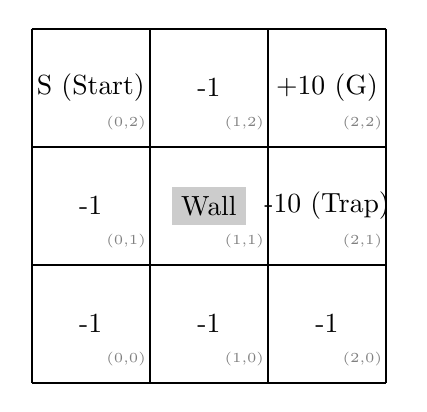
\begin{tikzpicture}[scale=1.5]
    \draw[thick] (0,0) grid (3,3);

    % States
    \node at (0.5, 2.5) {S (Start)};
    \node at (1.5, 2.5) {-1};
    \node at (2.5, 2.5) {+10 (G)};

    \node at (0.5, 1.5) {-1};
    \node[fill=black!20] at (1.5, 1.5) {Wall};
    \node at (2.5, 1.5) {-10 (Trap)};

    \node at (0.5, 0.5) {-1};
    \node at (1.5, 0.5) {-1};
    \node at (2.5, 0.5) {-1};

    % Coordinates labels
    \foreach \x in {0,1,2} \foreach \y in {0,1,2} \node[font=\tiny, gray] at (\x+0.8, \y+0.2) {(\x,\y)};
\end{tikzpicture}
\end{center}
States are denoted by $(x,y)$ where $x$ is column index (0-2) and $y$ is row index (0-2).
Start state $S$ is at $(0,2)$. Goal state $G$ is at $(2,2)$ with reward $+10$ (terminal).
The "Trap" at $(2,1)$ gives reward $-10$. All other transitions give reward $R=-1$.
Actions: Up, Down, Left, Right.
Assume $\gamma = 0.9$ and $\alpha = 0.5$.
Initial Q-values $Q(s,a) = 0$ for all states and actions.
Consider the following episode trajectory:
1. Start at $S(0,2)$. Agent chooses \textbf{Right}.
2. Lands in $(1,2)$, receives $R=-1$. From $(1,2)$, the agent's policy (e.g., $\epsilon$-greedy) chooses \textbf{Right} again.
3. However, before the update, we need to consider the algorithm.
\textbf{Scenario:}
The agent is at $S(0,2)$, takes action $A=$ Right, lands in $S'=(1,2)$, receives $R=-1$.
The agent then chooses the next action $A'$ from $S'$.
Suppose the greedy action at $S'$ is \textbf{Right} (towards Goal), but the exploratory action chosen is \textbf{Down} (towards Wall, stays in place or bounces).
Let's simplify:
\begin{itemize}
    \item $S = (0,2)$
    \item $A = \text{Right}$
    \item $R = -1$
    \item $S' = (1,2)$
    \item Greedy action at $S'$: $a^* = \text{Right}$ (leads to Goal, hypothetically best).
    \item Actual next action chosen $A' = \text{Down}$ (leads to Wall/Collision).
\end{itemize}
Note: For this problem, assume Q-values are initialized to 0. If multiple actions have max Q-value, ties are broken arbitrarily (say, Up $>$ Right $>$ Down $>$ Left).
Since all Q=0, $Q(S', \text{Right}) = 0$ and $Q(S', \text{Down}) = 0$.
So initially, the values don't distinguish.
Let's assume a pre-trained table where some values are learned to make the difference clear.
Suppose at $S'=(1,2)$:
\begin{itemize}
    \item $Q(S', \text{Right}) = 5.0$ (Learned path to goal)
    \item $Q(S', \text{Down}) = -2.0$ (Learned path to nowhere)
\end{itemize}
And at $S=(0,2)$, $Q(S, \text{Right}) = 1.0$.
\textbf{Task:}
Using the transition $S \xrightarrow{A=\text{Right}} S' (R=-1)$ and the next chosen action $A'=\text{Down}$:
\begin{enumerate}[label=(\alph*)]
    \item Calculate the updated $Q(S, \text{Right})$ using the \textbf{SARSA} update rule.
    \item Calculate the updated $Q(S, \text{Right})$ using the \textbf{Q-Learning} update rule.
    \item Explain the significance of the difference in these values in the context of "On-Policy" vs "Off-Policy" learning.
\end{enumerate}
\end{problem}
\begin{solution}
\textbf{Given Parameters:}
\begin{itemize}
    \item $\alpha = 0.5$, $\gamma = 0.9$
    \item Transition: $S=(0,2) \xrightarrow{\text{Right}} S'=(1,2)$, $R=-1$.
    \item Current Q-value: $Q(S, \text{Right}) = 1.0$.
    \item At $S'$, values are: $Q(S', \text{Right}) = 5.0$, $Q(S', \text{Down}) = -2.0$.
    \item Next actual action chosen: $A' = \text{Down}$.
\end{itemize}
\textbf{(a) SARSA Update}
SARSA (State-Action-Reward-State-Action) is an \textbf{On-Policy} algorithm. It updates the Q-value based on the action actually taken by the current policy ($A'$).
\[ Q(S, A) \leftarrow Q(S, A) + \alpha [ R + \gamma Q(S', A') - Q(S, A) ] \]
Substitute the values:
\begin{itemize}
    \item $Q(S', A') = Q(S', \text{Down}) = -2.0$.
\end{itemize}
\[ Q(S, \text{Right}) \leftarrow 1.0 + 0.5 [ -1 + 0.9(-2.0) - 1.0 ] \]
\[ Q(S, \text{Right}) \leftarrow 1.0 + 0.5 [ -1 - 1.8 - 1.0 ] \]
\[ Q(S, \text{Right}) \leftarrow 1.0 + 0.5 [ -3.8 ] \]
\[ Q(S, \text{Right}) \leftarrow 1.0 - 1.9 = -0.9 \]
The value decreased significantly because the agent actually took a bad action (Down) in the next state.
\textbf{(b) Q-Learning Update}
Q-Learning is an \textbf{Off-Policy} algorithm. It updates the Q-value based on the best possible action in the next state (Greedy), regardless of what action the agent actually takes.
\[ Q(S, A) \leftarrow Q(S, A) + \alpha [ R + \gamma \max_{a} Q(S', a) - Q(S, A) ] \]
Substitute the values:
\begin{itemize}
    \item $\max_{a} Q(S', a) = \max(Q(S', \text{Right}), Q(S', \text{Down}), \dots) = \max(5.0, -2.0) = 5.0$.
\end{itemize}
\[ Q(S, \text{Right}) \leftarrow 1.0 + 0.5 [ -1 + 0.9(5.0) - 1.0 ] \]
\[ Q(S, \text{Right}) \leftarrow 1.0 + 0.5 [ -1 + 4.5 - 1.0 ] \]
\[ Q(S, \text{Right}) \leftarrow 1.0 + 0.5 [ 2.5 ] \]
\[ Q(S, \text{Right}) \leftarrow 1.0 + 1.25 = 2.25 \]
The value increased because Q-Learning assumes the agent will act optimally from the next state onwards, ignoring the exploratory "mistake" (Down).
\textbf{(c) Significance}
The difference highlights the distinction between On-Policy and Off-Policy learning:
\begin{itemize}
    \item **SARSA** learns the value of the \textit{actual policy} being followed, including its exploration steps (epsilon-greedy). If the policy explores often (high epsilon) and takes dangerous actions (like 'Down' into a trap or wall), SARSA will propagate that risk back, lowering the Q-value of the previous state. It learns a "safer" path.
    \item **Q-Learning** learns the value of the \textit{optimal policy}, assuming that exploration is just a temporary anomaly. It is more aggressive/optimistic, learning the shortest path along the cliff edge because it assumes optimal behavior in the future, even if the current policy is likely to fall off.
\end{itemize}
\end{solution}
\newpage
\section{Value-Based Deep Reinforcement Learning}
\begin{problem}{Linear Value Function Approximation}
We wish to estimate the state-value function $V(s)$ using linear function approximation: $V(s) \approx \hat{v}(s, \mathbf{w}) = \mathbf{w}^\top \mathbf{x}(s)$, where $\mathbf{w}$ is a weight vector and $\mathbf{x}(s)$ is a feature vector representing state $s$.
We use the TD(0) algorithm with semi-gradient descent. The update rule is:
\[ \mathbf{w}_{t+1} = \mathbf{w}_t + \alpha [R_{t+1} + \gamma \hat{v}(S_{t+1}, \mathbf{w}_t) - \hat{v}(S_t, \mathbf{w}_t)] \nabla \hat{v}(S_t, \mathbf{w}_t) \]
**Given:**
\begin{itemize}
    \item Discount factor $\gamma = 0.9$, Step size $\alpha = 0.1$.
    \item Current weights $\mathbf{w}_t = [0.5, -0.2, 0.1]^\top$.
    \item Current state $S_t$ has features $\mathbf{x}(S_t) = [1, 0, 2]^\top$.
    \item Next state $S_{t+1}$ has features $\mathbf{x}(S_{t+1}) = [1, 1, 0]^\top$.
    \item Reward received $R_{t+1} = 2.0$.
\end{itemize}
\begin{enumerate}[label=(\alph*)]
    \item Calculate the estimated value of the current state $\hat{v}(S_t, \mathbf{w}_t)$.
    \item Calculate the estimated value of the next state $\hat{v}(S_{t+1}, \mathbf{w}_t)$.
    \item Calculate the TD Error $\delta_t$.
    \item Calculate the updated weight vector $\mathbf{w}_{t+1}$.
\end{enumerate}
\end{problem}
\begin{solution}
\textbf{(a) Estimate $\hat{v}(S_t, \mathbf{w}_t)$}
\[ \hat{v}(S_t, \mathbf{w}_t) = \mathbf{w}_t^\top \mathbf{x}(S_t) = (0.5)(1) + (-0.2)(0) + (0.1)(2) \]
\[ = 0.5 + 0 + 0.2 = 0.7 \]
\textbf{(b) Estimate $\hat{v}(S_{t+1}, \mathbf{w}_t)$}
\[ \hat{v}(S_{t+1}, \mathbf{w}_t) = \mathbf{w}_t^\top \mathbf{x}(S_{t+1}) = (0.5)(1) + (-0.2)(1) + (0.1)(0) \]
\[ = 0.5 - 0.2 + 0 = 0.3 \]
\textbf{(c) Calculate TD Error $\delta_t$}
The TD target is $R_{t+1} + \gamma \hat{v}(S_{t+1}, \mathbf{w}_t)$.
\[ \text{Target} = 2.0 + 0.9(0.3) = 2.0 + 0.27 = 2.27 \]
\[ \delta_t = \text{Target} - \hat{v}(S_t, \mathbf{w}_t) = 2.27 - 0.7 = 1.57 \]
\textbf{(d) Update Weights $\mathbf{w}_{t+1}$}
For linear approximation, the gradient is simply the feature vector: $\nabla \hat{v}(S_t, \mathbf{w}_t) = \mathbf{x}(S_t) = [1, 0, 2]^\top$.
\[ \mathbf{w}_{t+1} = \mathbf{w}_t + \alpha \delta_t \mathbf{x}(S_t) \]
\[ \mathbf{w}_{t+1} = \begin{bmatrix} 0.5 \\ -0.2 \\ 0.1 \end{bmatrix} + 0.1(1.57) \begin{bmatrix} 1 \\ 0 \\ 2 \end{bmatrix} \]
\[ \mathbf{w}_{t+1} = \begin{bmatrix} 0.5 \\ -0.2 \\ 0.1 \end{bmatrix} + \begin{bmatrix} 0.157 \\ 0 \\ 0.314 \end{bmatrix} \]
\[ \mathbf{w}_{t+1} = \begin{bmatrix} 0.657 \\ -0.2 \\ 0.414 \end{bmatrix} \]
\end{solution}
\newpage
\begin{problem}{Deep Q-Network (DQN) Backpropagation}
Consider a simple Deep Q-Network with one hidden layer.
\begin{center}
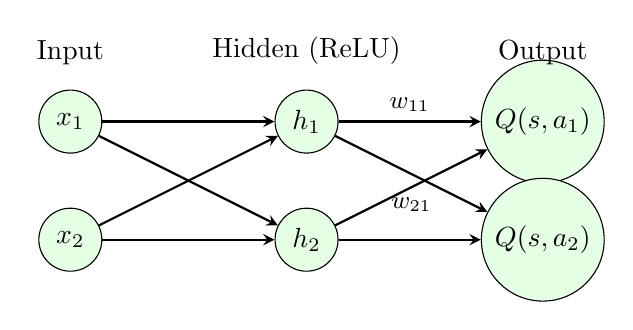
\begin{tikzpicture}[x=1.5cm, y=1.5cm]
    % Input Layer
    \node[netnode] (i1) at (0, 1) {$x_1$};
    \node[netnode] (i2) at (0, 0) {$x_2$};
    \node[above] at (0, 1.4) {Input};

    % Hidden Layer (ReLU)
    \node[netnode] (h1) at (2, 1) {$h_1$};
    \node[netnode] (h2) at (2, 0) {$h_2$};
    \node[above] at (2, 1.4) {Hidden (ReLU)};

    % Output Layer (Linear)
    \node[netnode] (o1) at (4, 1) {$Q(s, a_1)$};
    \node[netnode] (o2) at (4, 0) {$Q(s, a_2)$};
    \node[above] at (4, 1.4) {Output};

    % Connections
    \draw[arrow] (i1) -- (h1); \draw[arrow] (i1) -- (h2);
    \draw[arrow] (i2) -- (h1); \draw[arrow] (i2) -- (h2);

    \draw[arrow] (h1) -- node[above, font=\small] {$w_{11}$} (o1);
    \draw[arrow] (h1) -- (o2);
    \draw[arrow] (h2) -- node[below, font=\small] {$w_{21}$} (o1);
    \draw[arrow] (h2) -- (o2);
\end{tikzpicture}
\end{center}
\textbf{Scenario:}
\begin{itemize}
    \item Input state $s = [1, -1]$.
    \item Hidden layer weights (Input $\to$ Hidden) are fixed for this step.
    \item The computed hidden layer activations (after ReLU) are $h = [0.8, 0.5]$.
    \item Weights connecting Hidden to Output node 1 ($Q(s, a_1)$) are $\mathbf{w}_{out, 1} = [w_{11}, w_{21}]^\top = [1.5, -0.5]$.
    \item Bias terms are 0.
\end{itemize}
The agent took action $a_1$.
The environment returned reward $R = 1.0$ and next state $s'$.
The max Q-value calculated from the target network for the next state is $\max_{a'} Q(s', a'; \theta^-) = 2.0$.
Discount factor $\gamma = 0.9$.
\begin{enumerate}[label=(\alph*)]
    \item Calculate the predicted Q-value $Q(s, a_1)$.
    \item Calculate the TD Target $Y$.
    \item Calculate the Loss $L = \frac{1}{2}(Y - Q(s, a_1))^2$.
    \item Calculate the gradient of the Loss with respect to the weight $w_{11}$.
\end{enumerate}
\end{problem}
\begin{solution}
\textbf{(a) Predicted Q-value $Q(s, a_1)$}
The output is a linear combination of the hidden units:
\[ Q(s, a_1) = w_{11} h_1 + w_{21} h_2 \]
Given $h = [0.8, 0.5]$ and $\mathbf{w}_{out, 1} = [1.5, -0.5]$:
\[ Q(s, a_1) = (1.5)(0.8) + (-0.5)(0.5) \]
\[ = 1.2 - 0.25 = 0.95 \]
\textbf{(b) TD Target $Y$}
\[ Y = R + \gamma \max_{a'} Q(s', a'; \theta^-) \]
\[ Y = 1.0 + 0.9(2.0) = 1.0 + 1.8 = 2.8 \]
\textbf{(c) Loss $L$}
\[ L = \frac{1}{2}(Y - Q(s, a_1))^2 \]
\[ L = \frac{1}{2}(2.8 - 0.95)^2 = \frac{1}{2}(1.85)^2 \]
\[ L = \frac{1}{2}(3.4225) = 1.71125 \]
\textbf{(d) Gradient $\frac{\partial L}{\partial w_{11}}$}
Using the Chain Rule:
\[ \frac{\partial L}{\partial w_{11}} = \frac{\partial L}{\partial Q} \cdot \frac{\partial Q}{\partial w_{11}} \]
First part (Error term):
\[ \frac{\partial L}{\partial Q} = -(Y - Q(s, a_1)) = -(1.85) = -1.85 \]
(Note: commonly written as $(Q - Y)$ in gradient descent, but derivative of $\frac{1}{2}(Y-Q)^2$ wrt $Q$ is $-(Y-Q)$).
Second part (Input to weight):
\[ Q = w_{11} h_1 + w_{21} h_2 \implies \frac{\partial Q}{\partial w_{11}} = h_1 = 0.8 \]
Combine:
\[ \frac{\partial L}{\partial w_{11}} = (-1.85) \cdot (0.8) = -1.48 \]
\textit{Note: In a gradient descent update $w \leftarrow w - \alpha \nabla$, we would move the weight in the direction opposite to this gradient (i.e., increase the weight, which makes sense because our prediction 0.95 was lower than the target 2.8).}
\end{solution}
\newpage
\begin{problem}{Double DQN vs Standard DQN (Overestimation Bias)}
In Q-Learning and Standard DQN, the maximization step $\max_{a'} Q(s', a')$ can lead to overestimation of action values. Double DQN (DDQN) addresses this by decoupling action selection from action evaluation.
Consider a state $S'$ where the agent has 3 possible actions $\{a_1, a_2, a_3\}$.
We have two networks:
\begin{itemize}
    \item \textbf{Online Network ($\theta$):} Used to select actions.
    \item \textbf{Target Network ($\theta'$):} Used to evaluate values.
\end{itemize}
The Q-values estimated by both networks for state $S'$ are:
\begin{center}
\begin{tabular}{|c|c|c|}
\hline
Action & $Q(S', a; \theta)$ (Online) & $Q(S', a; \theta')$ (Target) \\
\hline
$a_1$ & 2.5 & 2.1 \\
$a_2$ & 3.0 & 1.5 \\
$a_3$ & 2.8 & 2.9 \\
\hline
\end{tabular}
\end{center}
Assume Reward $R = 1.0$ and $\gamma = 0.9$.
\begin{enumerate}[label=(\alph*)]
    \item Calculate the TD Target $Y_{DQN}$ using the \textbf{Standard DQN} formula.
    \item Calculate the TD Target $Y_{DDQN}$ using the \textbf{Double DQN} formula.
    \item Which method provides a lower estimate in this case? Explain why this is generally desirable.
\end{enumerate}
\end{problem}
\begin{solution}
\textbf{(a) Standard DQN Target}
Standard DQN uses the Target Network for both selection and evaluation (or historically just one network, but in modern DQN it uses the Target net for the max operator):
\[ Y_{DQN} = R + \gamma \max_{a} Q(S', a; \theta') \]
Looking at the Target Network column:
Values are $\{2.1, 1.5, 2.9\}$.
Max value is $2.9$ (for action $a_3$).
\[ Y_{DQN} = 1.0 + 0.9(2.9) = 1.0 + 2.61 = 3.61 \]
\textbf{(b) Double DQN Target}
Double DQN selects the best action using the \textit{Online} network, but evaluates its value using the \textit{Target} network.
\[ Y_{DDQN} = R + \gamma Q(S', \underset{a}{\text{argmax }} Q(S', a; \theta); \theta') \]
Step 1: Find best action using Online Network $\theta$.
Values are $\{2.5, 3.0, 2.8\}$.
Best action is $a^* = a_2$ (value 3.0).
Step 2: Evaluate this action $a_2$ using Target Network $\theta'$.
Look up $a_2$ in the Target column: $Q(S', a_2; \theta') = 1.5$.
Step 3: Calculate Target.
\[ Y_{DDQN} = 1.0 + 0.9(1.5) = 1.0 + 1.35 = 2.35 \]
\textbf{(c) Comparison}
$Y_{DQN} = 3.61$ vs $Y_{DDQN} = 2.35$.
Double DQN provides a significantly lower estimate.
This is desirable because noise in the estimates often causes the "max" operator to pick an action that is artificially high (overestimated) in the target network. By forcing the action choice to agree with the Online network (which might value a different action highly), we reduce the likelihood of propagating these maximum biases. In this specific example, the Online network thinks $a_2$ is best, but the Target network thinks $a_2$ is actually quite poor (1.5). Standard DQN would have ignored this disagreement and just taken the max of the Target (2.9), potentially training on a hallucinated high value.
\end{solution}
\newpage
\begin{problem}{Dueling DQN Architecture}
The Dueling DQN architecture separates the value of state $V(s)$ from the advantage of actions $A(s, a)$.
The final Q-value is combined using the formula:
\[ Q(s, a) = V(s) + \left( A(s, a) - \frac{1}{|A|} \sum_{a'} A(s, a') \right) \]
Suppose for a state $s$ with 3 actions $\{a_1, a_2, a_3\}$, the network streams output the following:
\begin{itemize}
    \item Value stream output: $V(s) = 10.0$
    \item Advantage stream outputs: $A(s, a_1) = 2.0$, $A(s, a_2) = -1.0$, $A(s, a_3) = 5.0$.
\end{itemize}
\begin{enumerate}[label=(\alph*)]
    \item Calculate the mean advantage $\bar{A}$.
    \item Calculate the final Q-values for all three actions: $Q(s, a_1)$, $Q(s, a_2)$, $Q(s, a_3)$.
    \item Verify that $V(s) \approx \frac{1}{|A|} \sum Q(s, a)$ is NOT necessarily true, but rather that the relative rank is preserved.
    \item What is the Q-value of the optimal action in this state?
\end{enumerate}
\end{problem}
\begin{solution}
\textbf{(a) Mean Advantage}
\[ \bar{A} = \frac{1}{3} (2.0 + (-1.0) + 5.0) = \frac{1}{3}(6.0) = 2.0 \]
\textbf{(b) Final Q-values}
Formula: $Q(s, a) = 10.0 + (A(s, a) - 2.0)$.
For $a_1$:
\[ Q(s, a_1) = 10.0 + (2.0 - 2.0) = 10.0 + 0 = 10.0 \]
For $a_2$:
\[ Q(s, a_2) = 10.0 + (-1.0 - 2.0) = 10.0 - 3.0 = 7.0 \]
For $a_3$:
\[ Q(s, a_3) = 10.0 + (5.0 - 2.0) = 10.0 + 3.0 = 13.0 \]
\textbf{(c) Verification}
The sum of advantages is forced to be zero in the aggregation.
Note that the Q-values are $10, 7, 13$. The optimal action is $a_3$ (13). The advantages were $2, -1, 5$ (optimal $a_3$). The rank is preserved.
\textbf{(d) Optimal Q-value}
$\max_a Q(s, a) = 13.0$.
\end{solution}
\newpage
\section{Policy Gradients \& Modern Architectures}
\begin{problem}{REINFORCE: Policy Gradient with Softmax}
Consider a policy $\pi(a|s, \theta)$ defined by a softmax distribution over action preferences $h(s, a, \theta) = \theta^T \phi(s, a)$.
For a single state $s$, there are 2 actions $a_1$ and $a_2$.
The feature vectors are:
\begin{itemize}
    \item $\phi(s, a_1) = [1, 0]^T$
    \item $\phi(s, a_2) = [0, 1]^T$
\end{itemize}
Current parameter vector $\theta = [0.5, 0.2]^T$.
Input state feature $\phi(s) = [1, 1]^T$ is not used directly, the preference is linear in action features.
The probabilities are given by:
\[ \pi(a|s) = \frac{e^{h(s, a)}}{\sum_{b} e^{h(s, b)}} \]
where $h(s, a) = \theta^T \phi(s, a)$.
\textbf{Scenario:}
The agent samples action $A_t = a_1$.
The return from this time step until the end of the episode is $G_t = 10.0$.
The baseline $b(s) = 0$ (for simplicity).
Step size $\alpha = 0.1$.
\begin{enumerate}[label=(\alph*)]
    \item Calculate the action preferences $h(s, a_1)$ and $h(s, a_2)$.
    \item Calculate the policy probabilities $\pi(a_1|s)$ and $\pi(a_2|s)$.
    \item Calculate the gradient of the log-probability $\nabla_\theta \ln \pi(A_t|s)$ for the chosen action $A_t = a_1$.
    \item Update the parameter vector $\theta$ using the REINFORCE update rule.
\end{enumerate}
\end{problem}
\begin{solution}
\textbf{(a) Action Preferences}
\[ h(s, a_1) = \theta^T \phi(s, a_1) = [0.5, 0.2] \cdot [1, 0]^T = 0.5 \]
\[ h(s, a_2) = \theta^T \phi(s, a_2) = [0.5, 0.2] \cdot [0, 1]^T = 0.2 \]
\textbf{(b) Policy Probabilities}
Compute exponentials:
\[ e^{0.5} \approx 1.6487 \]
\[ e^{0.2} \approx 1.2214 \]
Sum: $Z = 1.6487 + 1.2214 = 2.8701$.
\[ \pi(a_1|s) = \frac{1.6487}{2.8701} \approx 0.5744 \]
\[ \pi(a_2|s) = \frac{1.2214}{2.8701} \approx 0.4256 \]
\textbf{(c) Gradient of Log-Probability}
For softmax policy, the gradient is:
\[ \nabla_\theta \ln \pi(A_t|s) = \phi(s, A_t) - \sum_b \pi(b|s) \phi(s, b) \]
\[ = \phi(s, A_t) - \mathbb{E}_\pi[\phi(s, \cdot)] \]
Chosen action $A_t = a_1$.
$\phi(s, a_1) = [1, 0]^T$.
Expected feature vector:
\[ \mathbb{E}_\phi = 0.5744 [1, 0]^T + 0.4256 [0, 1]^T = [0.5744, 0.4256]^T \]
Gradient:
\[ \nabla \ln \pi(a_1|s) = [1, 0]^T - [0.5744, 0.4256]^T = [0.4256, -0.4256]^T \]
\textbf{(d) Parameter Update}
Update rule: $\theta_{t+1} = \theta_t + \alpha G_t \nabla \ln \pi(A_t|s)$.
\[ \theta_{t+1} = \begin{bmatrix} 0.5 \\ 0.2 \end{bmatrix} + 0.1(10.0) \begin{bmatrix} 0.4256 \\ -0.4256 \end{bmatrix} \]
\[ = \begin{bmatrix} 0.5 \\ 0.2 \end{bmatrix} + 1.0 \begin{bmatrix} 0.4256 \\ -0.4256 \end{bmatrix} \]
\[ = \begin{bmatrix} 0.9256 \\ -0.2256 \end{bmatrix} \]
The parameter for the chosen action ($a_1$, index 1) increased, and for the other action decreased.
\end{solution}
\newpage
\begin{problem}{One-Step Actor-Critic Update}
An Actor-Critic agent uses a linear Critic to estimate value $V(s, \mathbf{w}) = \mathbf{w}^T \mathbf{x}(s)$ and a softmax Actor $\pi(a|s, \mathbf{\theta})$.
\textbf{Current State $S_t$:}
Feature vector $\mathbf{x}(S_t) = [1, 2]^T$.
Critic weights $\mathbf{w} = [0.5, 0.1]^T$.
Value Estimate $V(S_t) = 0.5(1) + 0.1(2) = 0.7$.
\textbf{Transition:}
Action $A_t$ chosen.
Reward $R_{t+1} = 1.0$.
Next State $S_{t+1}$ feature vector $\mathbf{x}(S_{t+1}) = [1, 0]^T$.
Discount $\gamma = 0.9$.
\textbf{Actor Gradient:}
Assume we calculated the eligibility vector (gradient of log-prob) for the chosen action to be:
$\nabla_\theta \ln \pi(A_t|S_t) = [0.2, -0.1]^T$.
\begin{enumerate}[label=(\alph*)]
    \item Calculate the value of the next state $V(S_{t+1})$.
    \item Calculate the TD Error $\delta_t$.
    \item Update the Critic weights $\mathbf{w}$ (step size $\alpha_w = 0.1$).
    \item Update the Actor weights $\mathbf{\theta}$ (step size $\alpha_\theta = 0.1$).
\end{enumerate}
\end{problem}
\begin{solution}
\textbf{(a) Next State Value}
\[ V(S_{t+1}) = \mathbf{w}^T \mathbf{x}(S_{t+1}) = [0.5, 0.1] \cdot [1, 0]^T = 0.5 \]
\textbf{(b) TD Error}
\[ \delta_t = R_{t+1} + \gamma V(S_{t+1}) - V(S_t) \]
\[ \delta_t = 1.0 + 0.9(0.5) - 0.7 \]
\[ = 1.0 + 0.45 - 0.7 = 0.75 \]
\textbf{(c) Update Critic Weights}
Update rule: $\mathbf{w} \leftarrow \mathbf{w} + \alpha_w \delta_t \nabla V(S_t)$.
Gradient $\nabla V(S_t) = \mathbf{x}(S_t) = [1, 2]^T$.
\[ \mathbf{w}_{new} = [0.5, 0.1]^T + 0.1(0.75) [1, 2]^T \]
\[ = [0.5, 0.1]^T + 0.075 [1, 2]^T \]
\[ = [0.5, 0.1]^T + [0.075, 0.15]^T \]
\[ = [0.575, 0.25]^T \]
\textbf{(d) Update Actor Weights}
Update rule: $\mathbf{\theta} \leftarrow \mathbf{\theta} + \alpha_\theta \delta_t \nabla \ln \pi(A_t|S_t)$.
Assume initial $\mathbf{\theta}_{old} = [0, 0]^T$ (or just calculate the delta).
\[ \Delta \mathbf{\theta} = 0.1(0.75) [0.2, -0.1]^T \]
\[ = 0.075 [0.2, -0.1]^T = [0.015, -0.0075]^T \]
\end{solution}
\newpage
\begin{problem}{PPO Clipped Objective}
Proximal Policy Optimization (PPO) uses a clipped surrogate objective to prevent large policy updates.
\[ L^{CLIP}(\theta) = \mathbb{E}_t [ \min(r_t(\theta) \hat{A}_t, \text{clip}(r_t(\theta), 1-\epsilon, 1+\epsilon) \hat{A}_t) ] \]
where $r_t(\theta) = \frac{\pi_\theta(a_t|s_t)}{\pi_{\theta_{old}}(a_t|s_t)}$ is the probability ratio.
Let $\epsilon = 0.2$.
\textbf{Case 1 (Positive Advantage):}
\begin{itemize}
    \item Advantage $\hat{A}_t = 1.0$.
    \item Old prob $\pi_{old} = 0.4$.
    \item New prob $\pi_{new} = 0.5$.
\end{itemize}
\textbf{Case 2 (Negative Advantage):}
\begin{itemize}
    \item Advantage $\hat{A}_t = -1.0$.
    \item Old prob $\pi_{old} = 0.4$.
    \item New prob $\pi_{new} = 0.2$.
\end{itemize}
\begin{enumerate}[label=(\alph*)]
    \item Calculate the probability ratio $r_t$ for Case 1. Does clipping activate? Calculate the contribution to the loss.
    \item Calculate the probability ratio $r_t$ for Case 2. Does clipping activate? Calculate the contribution to the loss.
    \item Explain intuitively why PPO clips the objective in Case 1.
\end{enumerate}
\end{problem}
\begin{solution}
\textbf{(a) Case 1 (Positive Advantage)}
\[ r_t = \frac{0.5}{0.4} = 1.25 \]
We compute the two terms in the minimum:
1. Unclipped: $r_t \hat{A}_t = 1.25 \times 1.0 = 1.25$.
2. Clipped: $\text{clip}(1.25, 0.8, 1.2) \hat{A}_t$.
Since $1.25 > 1.2$, the term is clipped to $1.2$.
Value: $1.2 \times 1.0 = 1.2$.
Final Loss Contribution: $\min(1.25, 1.2) = 1.2$.
\textbf{Yes, clipping activates.}
\textbf{(b) Case 2 (Negative Advantage)}
\[ r_t = \frac{0.2}{0.4} = 0.5 \]
We compute the two terms:
1. Unclipped: $r_t \hat{A}_t = 0.5 \times (-1.0) = -0.5$.
2. Clipped: $\text{clip}(0.5, 0.8, 1.2) \hat{A}_t$.
Since $0.5 < 0.8$, the term is clipped to $0.8$.
Value: $0.8 \times (-1.0) = -0.8$.
Final Loss Contribution: $\min(-0.5, -0.8) = -0.8$.
\textbf{No, clipping does not activate (in the sense of the min operator).}
Wait, let's re-evaluate the min operator logic for negative numbers.
Unclipped: -0.5.
Clipped: -0.8.
$\min(-0.5, -0.8) = -0.8$.
Actually, the PPO objective is maximized (gradient ascent), but if we define Loss as something to minimize (descent), signs flip. The standard PPO paper maximizes the objective $L$.
Let's stick to Maximization language.
Objective value is $\min(-0.5, -0.8) = -0.8$.
So the objective is indeed the clipped version.
Wait, -0.8 is smaller than -0.5. So the min operator selects -0.8.
Does this make sense?
If Advantage is negative, we want to decrease probability ($r_t < 1$).
Here $r_t = 0.5$, we decreased it a lot.
The unclipped objective gain would be -0.5 (better than -0.8).
The clipped objective penalizes us more?
Actually, for negative advantage:
We want to decrease prob.
If $r_t$ goes below $1-\epsilon$, the clipped term stays at $(1-\epsilon)A = 0.8(-1) = -0.8$.
The unclipped term is $r_t A = 0.5(-1) = -0.5$.
Since $A < 0$, as $r_t$ decreases (good!), $r_t A$ increases (becomes less negative).
So $r_t A$ is the upper bound.
The min operator takes $\min(-0.5, -0.8) = -0.8$.
So the value is clamped at the lower value.
This seems correct. It effectively ignores changes that drive the ratio too far down?
Actually, PPO clipping for negative advantage is meant to preventing the ratio from going too close to 0 too fast?
No, the standard interpretation is:
If $A > 0$: we want to increase $r_t$. Clipping prevents $r_t$ from growing too large. $\min(r A, (1+\epsilon)A)$.
If $A < 0$: we want to decrease $r_t$. Clipping prevents $r_t$ from shrinking too small?
Let's check:
$\min(r A, (1-\epsilon)A)$. Since $A$ is negative, $(1-\epsilon)A$ is a negative number (e.g. -0.8). $r A$ is e.g. -0.5.
Min is -0.8.
Wait, if we take the gradient of -0.8 (constant), it is 0.
So if the ratio $r_t$ is below $1-\epsilon$ (0.8), the gradient is zero.
So we stop decreasing the probability.
Yes, that is the goal. We don't want to destroy the policy update by making probability 0.
So in this case, yes, the "clipping mechanism" (the lower bound) is active. The value returned is the clipped value.
\textbf{(c) Intuition for Case 1}
In Case 1, the action was good ($A > 0$), so we increased its probability ($r_t = 1.25$). However, PPO limits how much we can update the policy in a single step to ensure stability (Trust Region). Since $1.25 > 1 + \epsilon = 1.2$, we clip the objective. This means the gradient will be zero for further increases in $r_t$, preventing the policy from changing too drastically and potentially collapsing performance.
\end{solution}
\newpage
\begin{problem}{MCTS Trace (AlphaGo Style)}
Consider a Monte Carlo Tree Search process. We are at a node $S_0$.
The tree has the following structure and statistics $(W, N)$ where $W$ is total value and $N$ is visit count.
Root $S_0$: $N=10$.
Children of $S_0$:
\begin{itemize}
    \item $S_1$ (Action 1): $W=6, N=4$.
    \item $S_2$ (Action 2): $W=3, N=3$.
    \item $S_3$ (Action 3): $W=4, N=3$.
\end{itemize}
Exploration constant $c = 1.0$.
Formula: $UCB = \frac{W}{N} + c \sqrt{\frac{\ln N_{parent}}{N}}$.
\begin{enumerate}[label=(\alph*)]
    \item Calculate the UCB value for each child node ($S_1, S_2, S_3$).
    \item Which node is selected for the next simulation?
    \item Suppose we select the winner, perform a rollout, and get a result $v = +1$ (Win).
    \item Show the updated $(W, N)$ statistics for the path.
\end{enumerate}
\end{problem}
\begin{solution}
\textbf{(a) UCB Calculations}
$N_{parent} = 10$. $\ln(10) \approx 2.3026$.
Child $S_1$:
\[ \text{Exploit} = 6/4 = 1.5 \]
\[ \text{Explore} = 1.0 \sqrt{2.3026 / 4} = \sqrt{0.5756} \approx 0.7587 \]
\[ UCB_1 = 1.5 + 0.7587 = 2.2587 \]
Child $S_2$:
\[ \text{Exploit} = 3/3 = 1.0 \]
\[ \text{Explore} = 1.0 \sqrt{2.3026 / 3} = \sqrt{0.7675} \approx 0.876 \]
\[ UCB_2 = 1.0 + 0.876 = 1.876 \]
Child $S_3$:
\[ \text{Exploit} = 4/3 = 1.333 \]
\[ \text{Explore} = 1.0 \sqrt{2.3026 / 3} \approx 0.876 \]
\[ UCB_3 = 1.333 + 0.876 = 2.209 \]
\textbf{(b) Selection}
The node with the highest UCB value is $S_1$ (2.2587).
So, \textbf{$S_1$ is selected}.
\textbf{(c) Update}
We selected $S_1$.
Rollout result $v = +1$.
We update the statistics for $S_1$ and the Root $S_0$.
For $S_1$:
\[ N_{new} = 4 + 1 = 5 \]
\[ W_{new} = 6 + 1 = 7 \]
For Root $S_0$:
\[ N_{new} = 10 + 1 = 11 \]
% Note: Usually we don't track W for root for selection, but for completeness.
\[ W_{new} = \text{sum of children values} = \dots \]
Or simply update accumulated value:
\[ W_{root, new} = W_{root, old} + 1 \]
Updated Stats:
$S_1: (W=7, N=5)$.
$S_0: (N=11)$.
\end{solution}
\end{document}
